\chapter[Introduction]{\uppercase{Introduction}}
\label{chap:one}
The Chapter gets started with the history of Traditional Chinese
Medicine, and the modern digitization of wrist pulse diagnosis.
Due to the importance of wrist pulse features for analysis of illness,
there is a necessity to delve into the background and significance of
its case. 

\section{Background}
Chinese pulse diagnosis, one of the four diagnosis methods of
Traditional Chinese Medicine (TCM), namely inspection, `auscultation
and olfaction', inquiry and palpation, has been practiced for health
detection for more than 2000 years in China.\cite{Huynh1985,Flaws1995}
In the inspection
approach, TCM practitioners observe abnormal changes in the patient’s
vitality, color, appearance, secretions and excretions. The vital
signs encompass eyes, tongue, facial expressions, general and body
surface appearance. The inter-relationship between the external part
of the body such as face and tongue is used to
assist TCM practitioners to predict the pathological changes of
internal organs. Auscultation refers to listening of the patient’s
voice, breathing, and coughing and is used to judge the pathological
changes in the interior of the patient’s body, whereas olfaction
refers to smelling of secretion or excretion products. Inquiring or
interrogating is to query patient’s family history, feelings in
various aspects, e.g. chills and fever, perspiration, appetite and
thirst, as well as pain in term of its nature and locality. Palpation
approach involves pulse diagnosis. It contains profuse information of
the health condition of human body. 

From a hydrodynamics perspective, wrist pulse origins from the
disciplinary beats
of heart. In the view point of TCM, the heart is the main organ to perform
pulse, and the blood and breath air constitute the substantial
foundation of pulse. When the heart beats periodically between systole
and diastole, the blood ejected from left ventricle pounds the  
aorta valve and wall, generating a sort of vibration in a form of
waveform transmitting from the root of the aorta to any other
arteries, which is called \emph{Forward Wave}. If the forward wave is
affected by surrounding arterial branches, it reforms to the waveform
in the inverse direction, that is, \emph{Reflection Wave}. The
combination of both forms so-called pulse waveform.\cite{XiangheSong2008}
During the transmitting process, much body mechanism information has
been merged into the waveform. Thus They reflect the entire body function involved
with the breath activity of lung, the biochemistry of spleen,
evacuation of liver, and the warmth promotion of kidney. 
Besides, the wrist pulse is influenced by the cardiac status,
characteristics of the artery (including geometrical feature and
physical feature), vascular arguments, and other factors. Therefore,
the pulse diagnosis can provide important evidences for the feature
and trends of kinds of diseases. That is the reason why pulse
diagnosis is payed much attention to. 

Compared with Western Medicine (WM), traditional pulse diagnosis
also predominates on the cost of armarium. Western approaches
regularly requires sophisticated equipment or extensive chemical
processing, while in pulse diagnosis merely needs experience of
doctors. Table~\ref{tab:difftcmwm} shows a detailed comparison of them.
TCM diagnosis and treatments are popular in East Asia due to its low
cost. 

\begin{table}[htbp]
    \centering
    \renewcommand{\arraystretch}{1.5}
    \begin{tabular}{cp{0.4\textwidth}p{0.28\textwidth}} 
        \toprule[1.5pt]
        & Traditional Chinese Medicine & Western Medicine \\
        \midrule[1pt]
        Cost & Low & High \\
        Device & Simple & Sophisticated \\
        Foundation & Experience based & Evidence based \\
        Process & A summary of clinical observation & The result of
        laboratory experimentations \\
        Treatment & Herbs and nature agents & Chemical compounds \\
        Aims & Maintain health & Manage diseases \\
        Methodology & Inductive and synthetic & Reductive and
        analytical  \\
        \bottomrule[1.5pt]
    \end{tabular}
    \caption{Philosophical difference between Chinese and Western
    Medicine}
    \label{tab:difftcmwm}
\end{table}

However, fuzziness and uncertainty always are the two main problems impeding
the wide spread of TCM application. In thousand years of TCM
application, pulse practitioners relied on the imprecise information
from the fingertip feeling by touching the wrist of patient. Different
practitioners may not give identical results to the same patient.
Moreover, the attribution of pulse waveform expressed was usually
obscure. No standard was established to describe all types of pulses.
It eventually caused bifurcations in the traditional medicine. Pulse
diagnosis always requires a long experience, a comprehensive knowledge
base and a high level of skill of a doctor, and is subjective and
deficient in qualitative criteria of diagnosis. The instability and
fuzziness to some extent decrease the reliability and repeatability of
pulse diagnose. It is necessary to do researches concerning TCM
modernization by computerized techniques which allow researchers to
organize and analyze information more efficiently, more preciously
than the people-based fingertip feeling method. 



\section{Research objectives}
The objectification of human skin layer information has
experienced a long period. Such representative information as
continuous electrocardiogram (ECG), electroencephalogram (EEG),
electromyogram (EMG), respiratory wave and so on reflect
complementarily and directly the vital information of health
activities. Pulse research has been a long history and has firmer 
theory support, so it makes sense to further research. 

By the modernization of pulse diagnosis we can eliminate the
uncertainty and subjectivity from practitioners. Wrist pulse
assessment is a matter of technical skill and subjective experience,
\cite{hammer2001chinese} so the computerized analysis of digitalized pulse signal tends to
be more objective and persuasive.  The pulse 
image from data collection by devices shows a more precise and
objective information. New features that may not be perceived in
fingertips feeling method can be discovered to indicate diseases. 
Doctors could lightly distinguish the notch or abnormality in pulse
waveform from the computer screen rather than to conceptually describe
the wrist pulse in a form of metaphor. 

Although pulse diagnosis was gradually less used in the clinical
diagnosis in Western Medicine after the development of bacteriology
and anatomy, it is still widely applied in Chinese and India as an
auxiliary method. TCM now confronts a huge challenge in the modern
information era that prompts us do move forward objectification
of TCM. Moreover, pulse image gives a boost on physiology and
psychology as well as clinical pathology. 

So far, pulse objectification has scored a certain amount of
achievement. As a branch of biological
recognition architecture, computerized pulse diagnosis has effectively
binded traditional pulse diagnosis with modern information technology,
fulfilling a goal to automatically collection, processing, recognition
over pulse signals and final diagnosis of diseases. Pulse devices with
high resolution transducers are invented to collect pulse waveforms,
and save them into a database in favor of administration and review.
Consequently, digitalized pulse diagnosis plays an important ancillary
role in modern medicine due to its characteristics of painlessness,
harmlessness and real-time.\cite{Luo2007} 

With development of science and technology, such fields
bio-information, genetic engineering and nanotechnology and so forth
have derived profit from advanced equipments and approaches. The
combination of TCM and modern technology is an inevitable trend as
well. Hence, it is still a mission to utilize fruits of current
techniques to carry forward and further develop the legacy the
ancestors left.  

\section{Research status}
Pulse image represents the synthetic form
of changes on frequency, rhythm, sink-float, strength from the touch
and pressure sense when the doctor put his fingertips on patient’s
wrist. But the interpretation of Western Medicine on pulse image
merely rests on the analysis of features
such as frequency, rhythm, amplitude. Based on physiology, pathology
and local anatomy etc., WM deduces the position and reason of
pathology changes, rather than relating pulse image to the whole
organism. In this case, western local anatomy method is not suitable
for TCM objectification. In other words, the current study in the
western world betrayed the original goals of pulse image. There
remain India and Chinese employing the traditional pulse diagnosis
method yet. 

For the past many years, massive work on objectification of pulse
diagnosis has been done. Scholars in all parts of China has made
contribution to the objectification of pulse since 1950s.
\cite{zhang2005study,SunRen2006,CaiJun2007,ZHOUKuan-jiu2006,binghe2001fuzzy,liapplication,zhang2004feature}
Besides, scholars in other countries also has reached satisfactory
scores.\cite{yoon1987objective,michael1986instrument,yoon2000pulse,seng1977objectifying,wang1994alteration}

The objectification research of pulse diagnosis can be bifurcated into
two main aspects, the digitalized features analysis of pulse signals and
the designing of pulse collecting system. The digitalized features
analysis is the core of objectification process of pulse diagnosis,
and also the focal point of this paper. The designing of pulse
collecting system paves the foundation of the entire research. An
excellent result and discovery could not come out without a qualified
pulse collecting system. 

\subsection{The designing of pulse collecting system}
Some investigators upgraded merely a pulse transducer while some
others designed an integrated pulse analytical instrument. Both of
them are aspects of the pulse collecting system. Transducer plays a
crucial role on the result of final analysis, and eventually involves
the performance of whole system. In 1886, Vierordt first recorded
pulse image using sphygmograph based on lever and pressure. The
sphygmograph was not introduced into China until 1970s. After decades
of research, pulse sensors has significantly improved in precision,
sensitivity and repeatability.  There are mainly three types sensors
in common use at the present stage.
\begin{enumerate}
    \item Piezoresistance transducer. It is constructed on
        the property that resistivity is subject to variation of
        stresses. 
    \item Piezoelectric transducer. It transforms the pressure signal
        of pulse to electrical signal. 
    \item Piezomagnetic transducer. It is also called magnetoelastic
        transducer, which appeared in recent years. The operating
        principle is built on the basis of magnetoelastic effect, i.e.
        variation of pressure changes the magnetoconductivity of
        transducer, and then causes the change of electrical signal.
        However, limited to premature of related theory and
        technology, the piezomagnetic transducer failed to prevail. 
\end{enumerate}

Of course, There remains still other sorts of sensors, e.g. liquid sensor,
photoelectric sensor, strain pressure transducer, impedance sensor,
ultrasound sensor (Figure~\ref{fig:ultrasound}), PVDF sensor,
microphone transducer\cite{laub1983new}.
. On the other hand, with the development of computer
technology, all sorts of automated pulse electropulsographs were invented
to simplify the pulse data collecting process, like TP-CBS pulse
analyzer in Beijing, ZM-III electropulsograph by Shanghai University of
TCM, electropulsograph by Paik and Yoo in German. However, There is still a
long way to go for the development of pulse diagnosis device. 
\begin{figure}[htbp]
    \begin{center}
        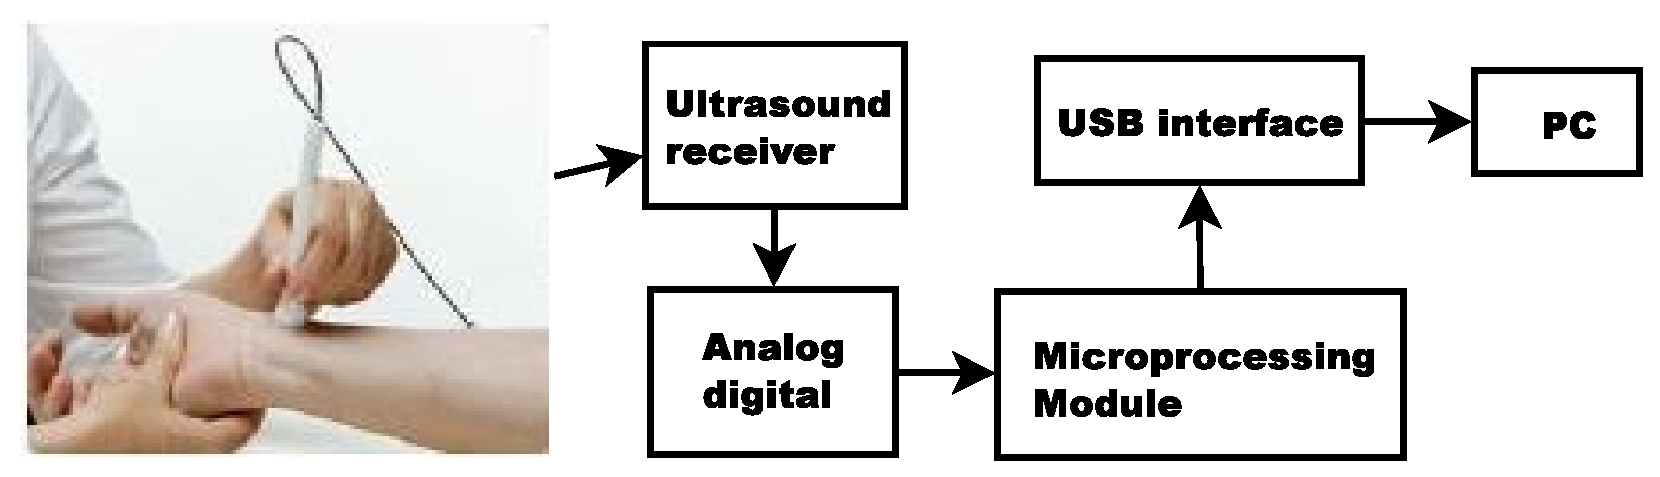
\includegraphics[width=0.7\textwidth]{ultrasound}
    \end{center}
    \caption{Pulse signal collection using ultrasonic blood analyzer}
    \label{fig:ultrasound}
\end{figure}
Aside from the diversity of sensor elements, the pattern of pulse
probes could be manifold, e.g. single position pattern, triple
positions pattern, multiple position pattern, rigid touch pattern,
soft touch pattern, in which single position pattern is the most
prevalent. Nevertheless, pulse probes trend to adopt triple positions
pattern. Multiple positions pattern or array pattern can eliminate the
accidental error from single point measurement. But how to collect and
analyze the extremely high dimentional information is still a problem.
The paper extends analysis upon pulse device with composite pressure and photoelectric
sensors. 

\subsection{The analysis and diagnosis objectified digital features}
Raw pulse data from the pulse sensors is not suitable for direct
analysis. Instead, it should be preprocessed first. The analysis of
pulse digital features mainly is separated into two steps, i.e. signal
processing and pattern classification. The signal
processing of pulse mainly solves the interference from high frequency
noise, pseudo-peaks, baseline drift, and classifies and verifies the
pulse signal by extracting feature argument from the waveform. 

Then some diagnosis features that manage to reflect the
characteristics of pulse signal are extracted, which can be
time-domain, frequency-domain features and time-frequency
features.\cite{zhang2005study,leonard2004wavelet,zhang2002wavelet, lu1999pulse,zhang2008wavelet,chen2011computerized}
 For example, Leonard et al.\cite{leonard2004wavelet} revealed that it is possible to
distinguish healthy and unwell children by using wavelet power
features and wavelet entropy of the pulse signal. Zhang et al.\cite{zhang2002wavelet}
proposed a wavelet transform based method to extract features from
carotid blood flow signals, and used a back-propagation (BP) neural
network to make the classification among 30 samples. Moreover, Zhang
et al.\cite{zhang2008wavelet} used the wavelet method to extract different pulse
features, including wavelet powers, wavelet packet powers and Doppler
ultrasonic diagnostic parameters. Although some of the above methods
have achieved encouraging results, their effectiveness are still
subject to further assessment due to the limited number of samples and
types of diseases. For example, in Leonard’s research,\cite{leonard2004wavelet} only 20
samples are used to distinguish well and unwell children, while in
Zhang’s research,\cite{zhang2008wavelet} two kinds of diseases are investigated. 

In view of the pulse research centered on linear method, nonlinear
dynamics as the third revolution of physics in this century is
gradually applied on the pulse feature extraction. At present,
nonlinear methods perform well on bio-signal to some extent for that
the human body is a nonlinear system, an integral constituted by time
and space. Consequently, a couple of methods based on nonlinear
dynamics are used to research the law of
pulse.\cite{li1999study,rauchberger1998analysis,barreto1997adaptive,naschitz2003assessment}
Wang primarily studied on the pulse mutation\cite{li1999study} and Rauchberger et al. studies on
the quotidian variation of pulse.\cite{rauchberger1998analysis} Armando et al. devised an
adapted method of plethysmography to amplify signals.\cite{barreto1997adaptive} Moreover,
Naschitz et al. used fractal and recursive graph to analyze the
transmission time of pulse.\cite{naschitz2003assessment}

When it comes to the next stage pattern classification, major methods
such as multi-factor pulse image recognition, syntactic pattern
recognition, adapted auto-regression modeling, fuzzy logic, clustering
analysis, neural network method etc. are widely used. For example,
Allen found that neural network method archived the best result
comparing with linear discriminant method and K-neighbor method. 
Chen et al.\cite{chen2009wrist} introduced Fuzzy C-Means (FCM) which aims, as a most
widely used algorithm for statistical data analysis, to cluster two or
more data point groups into clusters so that items in the same class
are as similar as possible and items in different classes are
dissimilar as possible, and found the use of membership function in
FCM that means an object can belong an object several clusters at the
same time but with different degrees is important for disease
analysis. Some other researchers\cite{zhang2005study,lu1999pulse} also proved that it is
possible to identify human sub-health status based on pulse signals by
using linear discriminate classifier. 

In summary, the research status of computerized pulse has not yet
formulated a standard to describe completely the 28 traditional pulse
types by digital features. The formation of pulse is actually so
complicated that solo sensor cannot represent the precise information
of pulse, instead fusion of multi-sensors become more effective.
Moreover, such factors as the repeatability of pulse collection, the
precise position of pulse, the pressure of probe are all basic
problems that we need solve. The established analysis of pulse image
only relies on time domain, frequency domain and simple clustering
that more incisive feature extraction method is required. Another
problem is that the objectified pulse has not been well associated
with concrete disease in clinical diagnosis. Combining with other
diagnosis method such as ECG, tongue color, oral smell makes it more
precise for prognosis as well. 

\section{Thesis organization}

Fig.~\ref{fig:outline} shows the outline of this thesis. First, pulse
data of patients with disparate health condition is gathered in
Guangdong hospital of Tradition Chinese Medicine, based
on an independent pulse detecting and collecting device with fusion of
pressure and photoelectric transducers, and then organized as the
database for later research. Second, de-noising algorithms are
introduced to detect and remove pseudo-peaks and singulars. Third, a
new series of features proposed helps the discrimination of diseases.
Finally, several classifiers are used to evaluate the
representativeness of features.

\begin{figure}[htpb]
    \begin{center}
        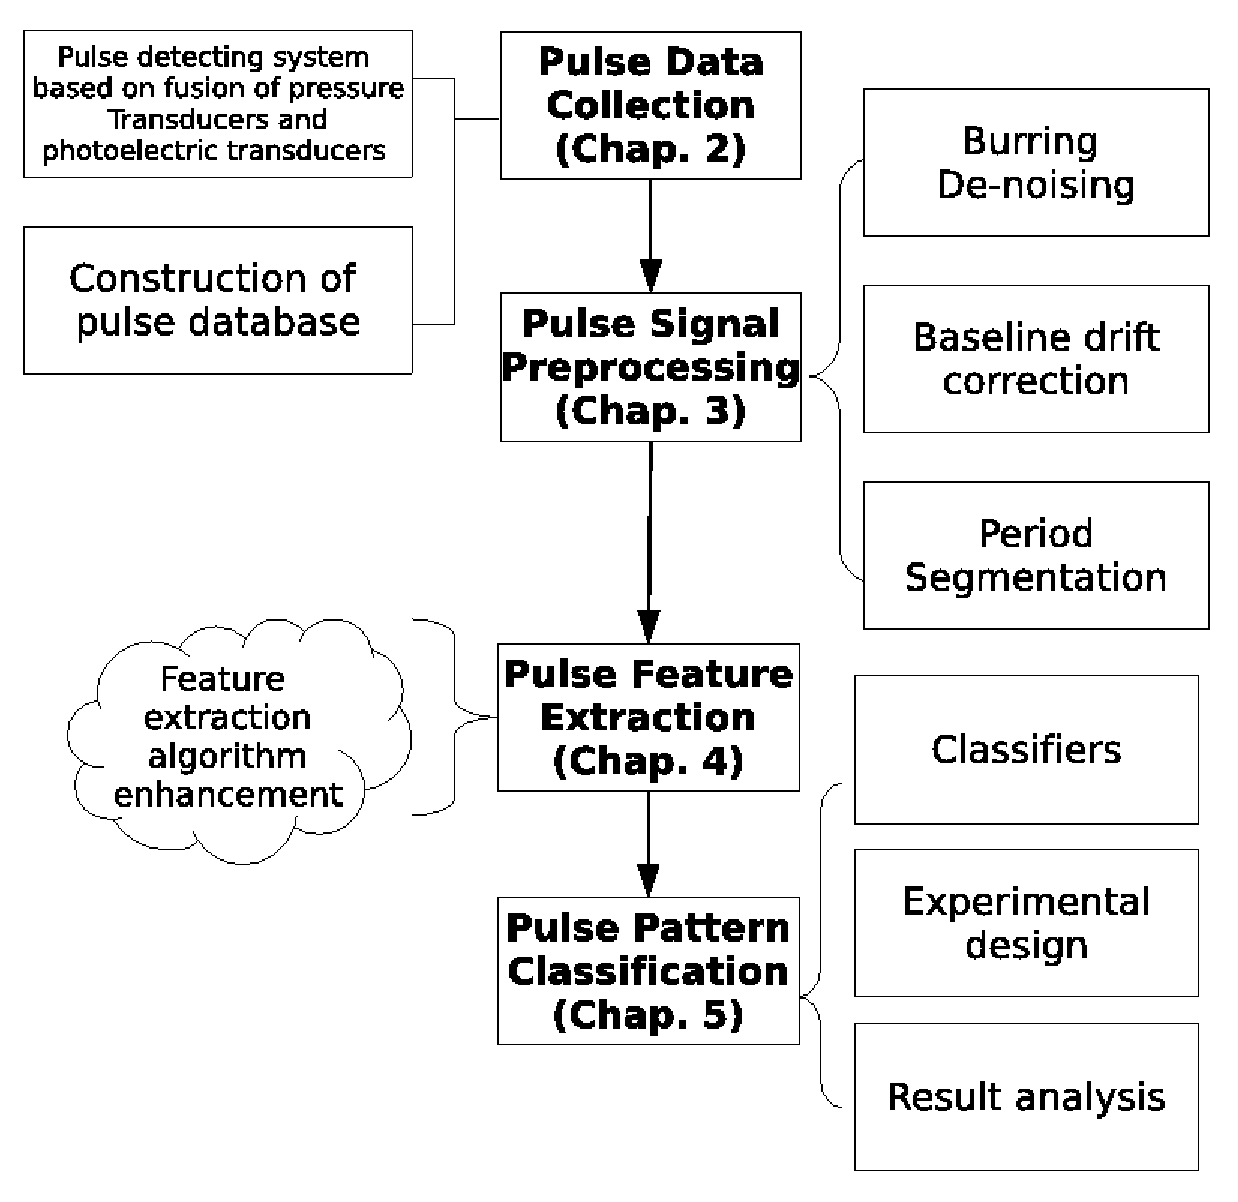
\includegraphics[width=0.8\textwidth]{outline}
    \end{center}
    \caption{Outline of this thesis}
    \label{fig:outline}
\end{figure}

The main content of the paper is organized as follows. 

Chapter~\ref{chap:one} introduces the background of pulse diagnosis
and related research status.

Chapter~\ref{chap:two} describes the principle and basic structure of pressure sensors and
photoelectric sensors based pulse collecting system, and
how to gather wrist pulse data from patients in the hospital. After
that, information is well ordered and saved as an integrated database. 

Chapter~\ref{chap:three} presents a succession of algorithms to 
remove abnormality and smooth the pulse waveforms. First, a
high-frequent burr due to the electromagnetic interference of the
device power is adulterated into the pulse signal, which urges the wavelet
1-D noise filter to smooth. Second, An unknown noise is discovered and
gotten rid of using low-pass linear filter. Third, a wavelet-based
cascaded adaptive filter helps remove the baseline drift problem
occurred during the sampling process. Finally, single periodical
waveform is cut out for further analysis. 

Chapter~\ref{chap:four} illustrates improved time-domain features and
other-domain features extracted. \todo{}

Chapter~\ref{chap:five} compares the performance of features under
three classifiers, i.e. support vector machine (SVM), Linear
Discriminant analysis (LDA), K-nearest neighbor (KNN). \todo{}

In the end, the essay makes a conclusion to summarize and evaluate the
work and addresses the prospect of pulse objectification. 


